\documentclass[]{article}
\usepackage{lmodern}
\usepackage{amssymb,amsmath}
\usepackage{ifxetex,ifluatex}
\usepackage{fixltx2e} % provides \textsubscript
\ifnum 0\ifxetex 1\fi\ifluatex 1\fi=0 % if pdftex
  \usepackage[T1]{fontenc}
  \usepackage[utf8]{inputenc}
\else % if luatex or xelatex
  \ifxetex
    \usepackage{mathspec}
  \else
    \usepackage{fontspec}
  \fi
  \defaultfontfeatures{Ligatures=TeX,Scale=MatchLowercase}
  \newcommand{\euro}{€}
\fi
% use upquote if available, for straight quotes in verbatim environments
\IfFileExists{upquote.sty}{\usepackage{upquote}}{}
% use microtype if available
\IfFileExists{microtype.sty}{%
\usepackage{microtype}
\UseMicrotypeSet[protrusion]{basicmath} % disable protrusion for tt fonts
}{}
\usepackage[margin=1in]{geometry}
\usepackage{hyperref}
\PassOptionsToPackage{usenames,dvipsnames}{color} % color is loaded by hyperref
\hypersetup{unicode=true,
            pdftitle={Binary Models},
            pdfborder={0 0 0},
            breaklinks=true}
\urlstyle{same}  % don't use monospace font for urls
\usepackage{color}
\usepackage{fancyvrb}
\newcommand{\VerbBar}{|}
\newcommand{\VERB}{\Verb[commandchars=\\\{\}]}
\DefineVerbatimEnvironment{Highlighting}{Verbatim}{commandchars=\\\{\}}
% Add ',fontsize=\small' for more characters per line
\usepackage{framed}
\definecolor{shadecolor}{RGB}{248,248,248}
\newenvironment{Shaded}{\begin{snugshade}}{\end{snugshade}}
\newcommand{\KeywordTok}[1]{\textcolor[rgb]{0.13,0.29,0.53}{\textbf{{#1}}}}
\newcommand{\DataTypeTok}[1]{\textcolor[rgb]{0.13,0.29,0.53}{{#1}}}
\newcommand{\DecValTok}[1]{\textcolor[rgb]{0.00,0.00,0.81}{{#1}}}
\newcommand{\BaseNTok}[1]{\textcolor[rgb]{0.00,0.00,0.81}{{#1}}}
\newcommand{\FloatTok}[1]{\textcolor[rgb]{0.00,0.00,0.81}{{#1}}}
\newcommand{\ConstantTok}[1]{\textcolor[rgb]{0.00,0.00,0.00}{{#1}}}
\newcommand{\CharTok}[1]{\textcolor[rgb]{0.31,0.60,0.02}{{#1}}}
\newcommand{\SpecialCharTok}[1]{\textcolor[rgb]{0.00,0.00,0.00}{{#1}}}
\newcommand{\StringTok}[1]{\textcolor[rgb]{0.31,0.60,0.02}{{#1}}}
\newcommand{\VerbatimStringTok}[1]{\textcolor[rgb]{0.31,0.60,0.02}{{#1}}}
\newcommand{\SpecialStringTok}[1]{\textcolor[rgb]{0.31,0.60,0.02}{{#1}}}
\newcommand{\ImportTok}[1]{{#1}}
\newcommand{\CommentTok}[1]{\textcolor[rgb]{0.56,0.35,0.01}{\textit{{#1}}}}
\newcommand{\DocumentationTok}[1]{\textcolor[rgb]{0.56,0.35,0.01}{\textbf{\textit{{#1}}}}}
\newcommand{\AnnotationTok}[1]{\textcolor[rgb]{0.56,0.35,0.01}{\textbf{\textit{{#1}}}}}
\newcommand{\CommentVarTok}[1]{\textcolor[rgb]{0.56,0.35,0.01}{\textbf{\textit{{#1}}}}}
\newcommand{\OtherTok}[1]{\textcolor[rgb]{0.56,0.35,0.01}{{#1}}}
\newcommand{\FunctionTok}[1]{\textcolor[rgb]{0.00,0.00,0.00}{{#1}}}
\newcommand{\VariableTok}[1]{\textcolor[rgb]{0.00,0.00,0.00}{{#1}}}
\newcommand{\ControlFlowTok}[1]{\textcolor[rgb]{0.13,0.29,0.53}{\textbf{{#1}}}}
\newcommand{\OperatorTok}[1]{\textcolor[rgb]{0.81,0.36,0.00}{\textbf{{#1}}}}
\newcommand{\BuiltInTok}[1]{{#1}}
\newcommand{\ExtensionTok}[1]{{#1}}
\newcommand{\PreprocessorTok}[1]{\textcolor[rgb]{0.56,0.35,0.01}{\textit{{#1}}}}
\newcommand{\AttributeTok}[1]{\textcolor[rgb]{0.77,0.63,0.00}{{#1}}}
\newcommand{\RegionMarkerTok}[1]{{#1}}
\newcommand{\InformationTok}[1]{\textcolor[rgb]{0.56,0.35,0.01}{\textbf{\textit{{#1}}}}}
\newcommand{\WarningTok}[1]{\textcolor[rgb]{0.56,0.35,0.01}{\textbf{\textit{{#1}}}}}
\newcommand{\AlertTok}[1]{\textcolor[rgb]{0.94,0.16,0.16}{{#1}}}
\newcommand{\ErrorTok}[1]{\textcolor[rgb]{0.64,0.00,0.00}{\textbf{{#1}}}}
\newcommand{\NormalTok}[1]{{#1}}
\usepackage{longtable,booktabs}
\usepackage{graphicx,grffile}
\makeatletter
\def\maxwidth{\ifdim\Gin@nat@width>\linewidth\linewidth\else\Gin@nat@width\fi}
\def\maxheight{\ifdim\Gin@nat@height>\textheight\textheight\else\Gin@nat@height\fi}
\makeatother
% Scale images if necessary, so that they will not overflow the page
% margins by default, and it is still possible to overwrite the defaults
% using explicit options in \includegraphics[width, height, ...]{}
\setkeys{Gin}{width=\maxwidth,height=\maxheight,keepaspectratio}
\setlength{\parindent}{0pt}
\setlength{\parskip}{6pt plus 2pt minus 1pt}
\setlength{\emergencystretch}{3em}  % prevent overfull lines
\providecommand{\tightlist}{%
  \setlength{\itemsep}{0pt}\setlength{\parskip}{0pt}}
\setcounter{secnumdepth}{5}

%%% Use protect on footnotes to avoid problems with footnotes in titles
\let\rmarkdownfootnote\footnote%
\def\footnote{\protect\rmarkdownfootnote}

%%% Change title format to be more compact
\usepackage{titling}

% Create subtitle command for use in maketitle
\newcommand{\subtitle}[1]{
  \posttitle{
    \begin{center}\large#1\end{center}
    }
}

\setlength{\droptitle}{-2em}
  \title{Binary Models}
  \pretitle{\vspace{\droptitle}\centering\huge}
  \posttitle{\par}
  \author{}
  \preauthor{}\postauthor{}
  \date{}
  \predate{}\postdate{}


% Redefines (sub)paragraphs to behave more like sections
\ifx\paragraph\undefined\else
\let\oldparagraph\paragraph
\renewcommand{\paragraph}[1]{\oldparagraph{#1}\mbox{}}
\fi
\ifx\subparagraph\undefined\else
\let\oldsubparagraph\subparagraph
\renewcommand{\subparagraph}[1]{\oldsubparagraph{#1}\mbox{}}
\fi


\usepackage{amsthm}
\newtheorem{theorem}{Theorem}[section]
\newtheorem{lemma}{Lemma}[section]
\theoremstyle{definition}
\newtheorem{definition}{Definition}[section]
\newtheorem{corollary}{Corollary}[section]
\newtheorem{proposition}{Proposition}[section]
\theoremstyle{definition}
\newtheorem{example}{Example}[section]
\theoremstyle{remark}
\newtheorem*{remark}{Remark}
\begin{document}
\maketitle

{
\setcounter{tocdepth}{2}
\tableofcontents
}
\section{Introduction}\label{introduction}

Many questions we seek to answer in social science research are binary:
Will the Tories win the next election? Will Brexit help or hurt the
economy? Will a country go to war? To shed light on these kinds of
questions, we employ logistic regression. In this workshop we cover the
theory of regression with a binary dependent variable and then turn to
the practical application in R. We will estimate our own logistic
regression, show by how much our model improves upon prior knowledge and
illustrate our results such that an audience without statistical
knowledge can interpret the results. Students should be familiar with R
as well as basic concepts of statistics such as the level of measurement
of a variable, the mean and linear regression.

We cover the following:

\begin{itemize}
\tightlist
\item
  Theory of regression with a binary dependent variable
\item
  Estimating a logistic regression in R
\item
  Assessing the quality of our model
\item
  Making predictions based on our model
\end{itemize}

\begin{center}\rule{0.5\linewidth}{\linethickness}\end{center}

\emph{Last Updated: May 24, 2017 7:36 PM}

\section{Binary Models -- Logit and
Probit}\label{binary-models-logit-and-probit}

Binary dependent variables are frequent in social science
research\ldots{}

\begin{itemize}
\tightlist
\item
  \ldots{} why does somebody vote or not?
\item
  \ldots{} why does a country go to war or not?
\item
  \ldots{} why does a legislator vote \emph{yes} or \emph{no}?
\item
  \ldots{} why do some countries have the death penalty and other not?
\end{itemize}

\subsection{The Linear Probability
Model}\label{the-linear-probability-model}

The linear probability model relies on linear regression to analyze
binary variables.

\begin{eqnarray}
y_i & = & \beta_0 + \beta_1 \cdot x_{1i} + \beta_2 \cdot x_{2i}+ ... + \beta_k \cdot x_{ki} + \varepsilon_{i}\\
Pr(y_i=1|x_1, x_2, ...) & = & \beta_0 + \beta_1 \cdot x_{1i} + \beta_2 \cdot x_{2i}+ ... + \beta_k \cdot x_{ki} \\
\end{eqnarray}

\subsubsection{Advantages}\label{advantages}

\begin{itemize}
\tightlist
\item
  We can use a well-known model for a new class of phenomena
\item
  Easy to interpret the marginal effects of \(x\) variables
\end{itemize}

\subsubsection{Disadvantages}\label{disadvantages}

The linear model needs a continuous dependent variable, if the dependent
variable is binary we run into problems:

\begin{itemize}
\item
  Predictions, \(\hat y\), are interpreted as probability for \(y=1\)\\
  {[}\(\rightarrow\) \(P(y=1) = \hat y = \beta_0\)+\(\beta_1 x\), can be
  above 1 if \(x\) is large enough{]}\{\}\\
  {[}\(\rightarrow\) \(P(y=0) = 1- \hat y = 1 - \beta_0\)+\(\beta_1 x\),
  can be below 0 if \(x\) is small enough{]}\{\}
\item
  The errors will not have a constant variance.\\
  {[}\(\rightarrow\) For a given \(x\) the residual can be either
  (1-\(\beta_0\)-\(\beta_1 x\)) or (\(\beta_0\)+\(\beta_1 x\)){]}\{\}
\item
  The linear function might be wrong\\
  {[}\(\rightarrow\) Imagine you buy a car. Having an additional
  £1000~has a very different effect if you are broke or if you already
  have another £12,000~for a car.{]}\{\}
\end{itemize}

\textbf{Predictions can lay outside \(I=[0,1]\)}

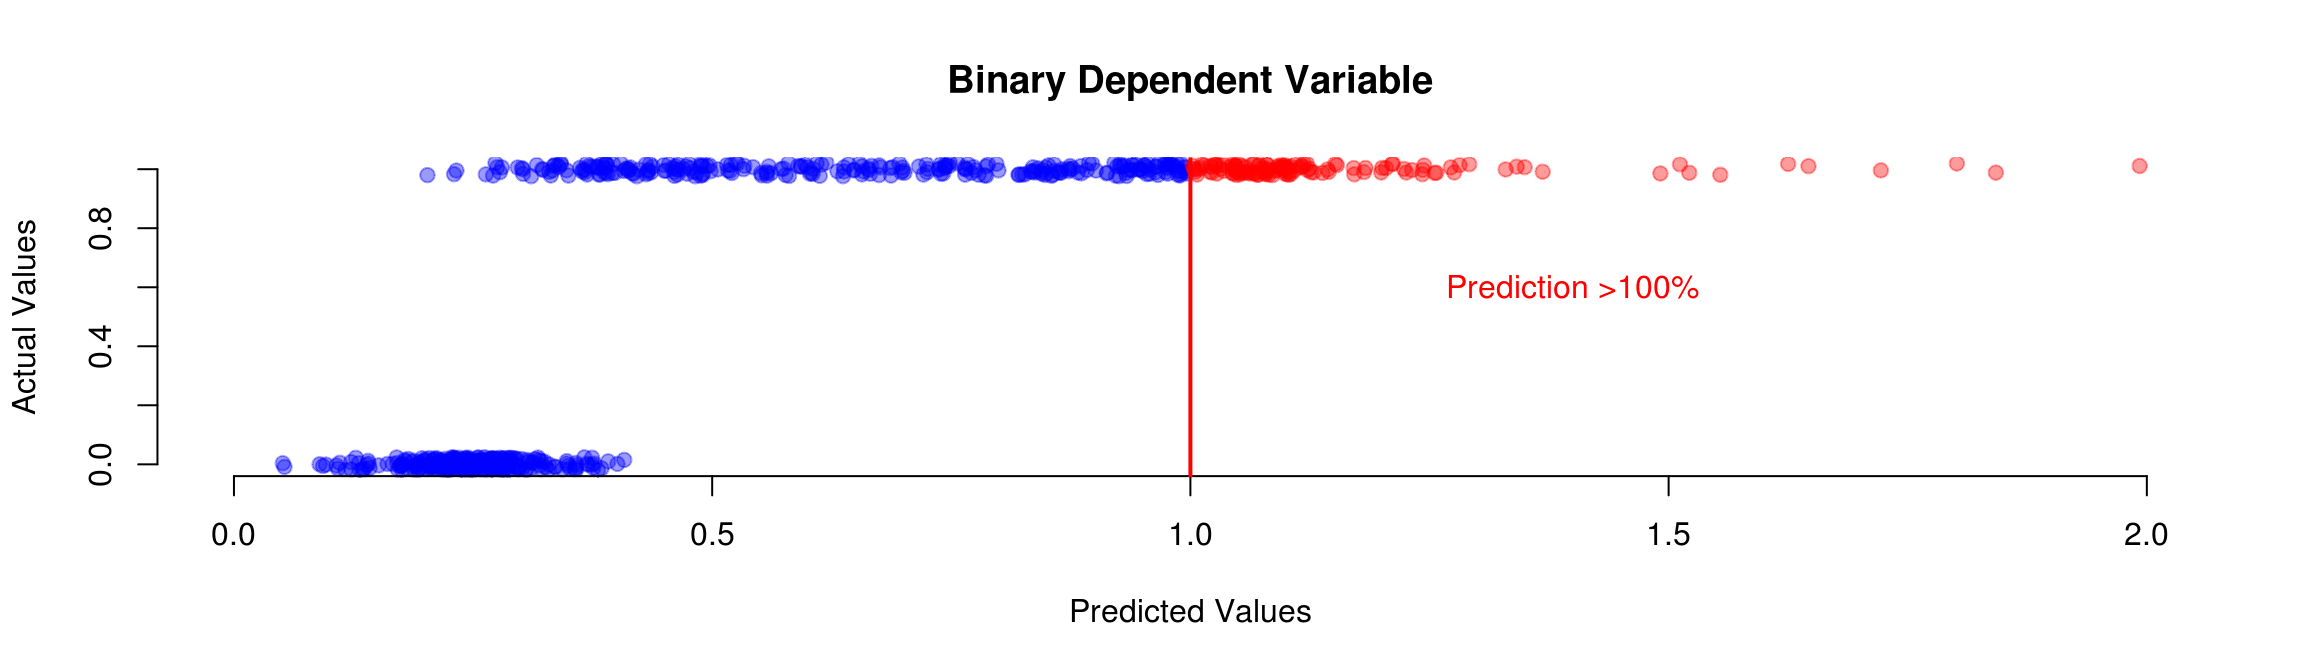
\includegraphics{_main_files/figure-latex/unnamed-chunk-2-1.pdf}

\textbf{Residuals if the dependent variable is binary:}

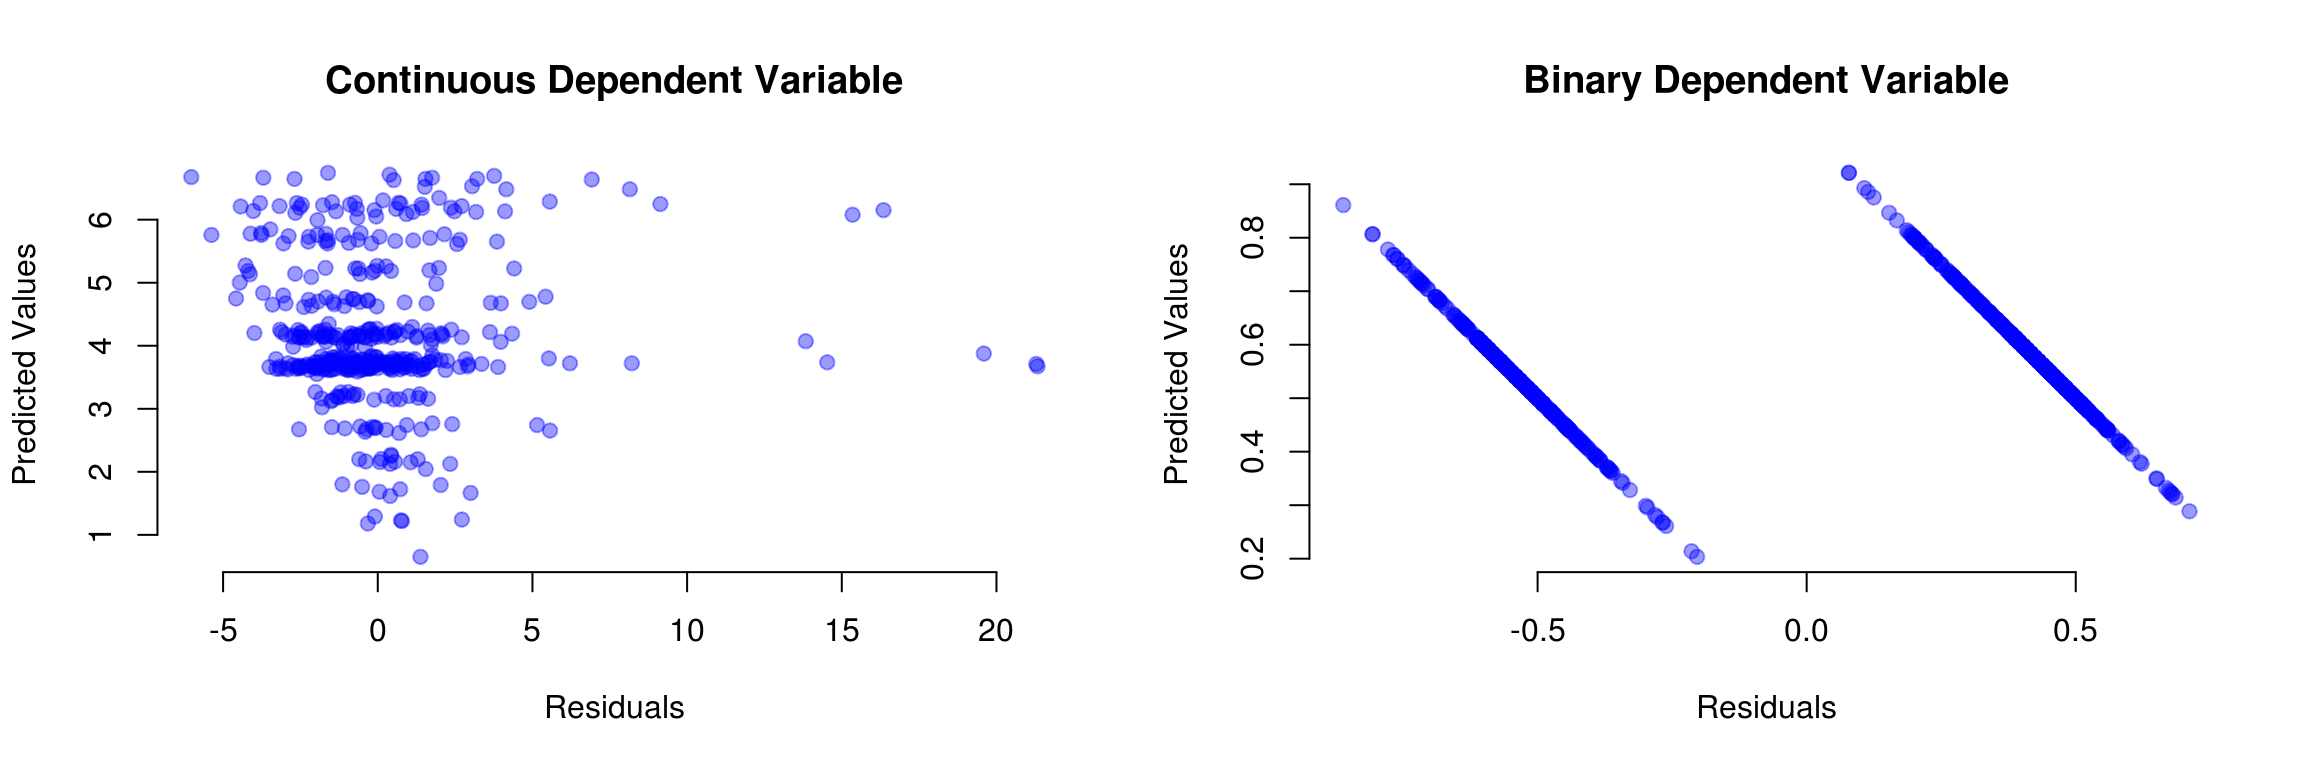
\includegraphics{_main_files/figure-latex/unnamed-chunk-3-1.pdf}

\subsection{Building a Model from Probability
Theory}\label{building-a-model-from-probability-theory}

\begin{itemize}
\tightlist
\item
  We want to make predictions in terms of probability
\item
  We can have a model like this: \(P(y_i=1)={F(\beta_0 + \beta_1 x_i)}\)
  where \(F(\cdot)\) should be a function which never returns values
  below 0 or above 1
\item
  There are two possibilities for \(F(\cdot)\): cumulative normal
  (\(\Phi\)) or logistic (\(\Delta\)) distribution
\end{itemize}

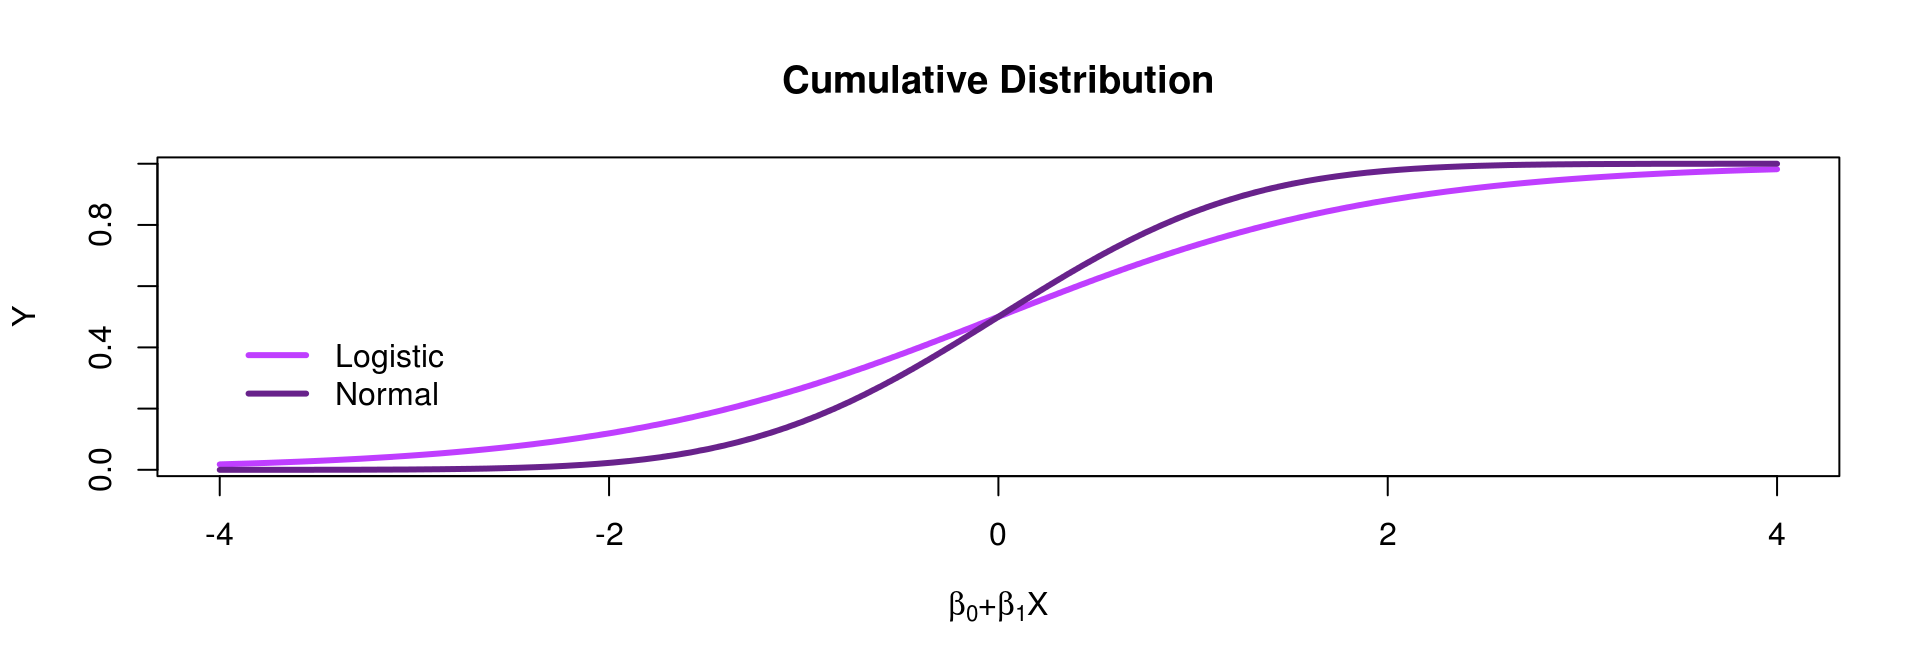
\includegraphics{_main_files/figure-latex/unnamed-chunk-4-1.pdf}

\subsection{Logit and Probit}\label{logit-and-probit}

\begin{itemize}
\item
  We now have a model where \(\hat y \in [0,1]\)\\
  \(\rightarrow\) All predictions are probabilities
\item
  We have two possible models to use\\
  {[}\(\rightarrow\) The logit model is based on the cumulative logistic
  distribution (\(\Delta\)){]}\{\}\\
  {[}\(\rightarrow\) The probit model is based on the cumulative normal
  distribution (\(\Phi\)){]}\{\}
\end{itemize}

We will use logit more often because we can write
\(\Delta(x) = \frac{1}{1 + \exp(-x)}\),\\
while probit models are tricky:
\(\Phi(x) = \int_{-\infty}^{x}\frac{1}{\sqrt{2\pi}}\exp(\frac{-(x)^2}{2}) dx\)

\subsection{Logit Model}\label{logit-model}

The logit model is then:
\(P(y_i=1)=\frac{1}{1 + \exp(-\beta_0 - \beta_1 x_i)}\)

For \(\beta_0 = 0\) and \(\beta_1=2\) we get:

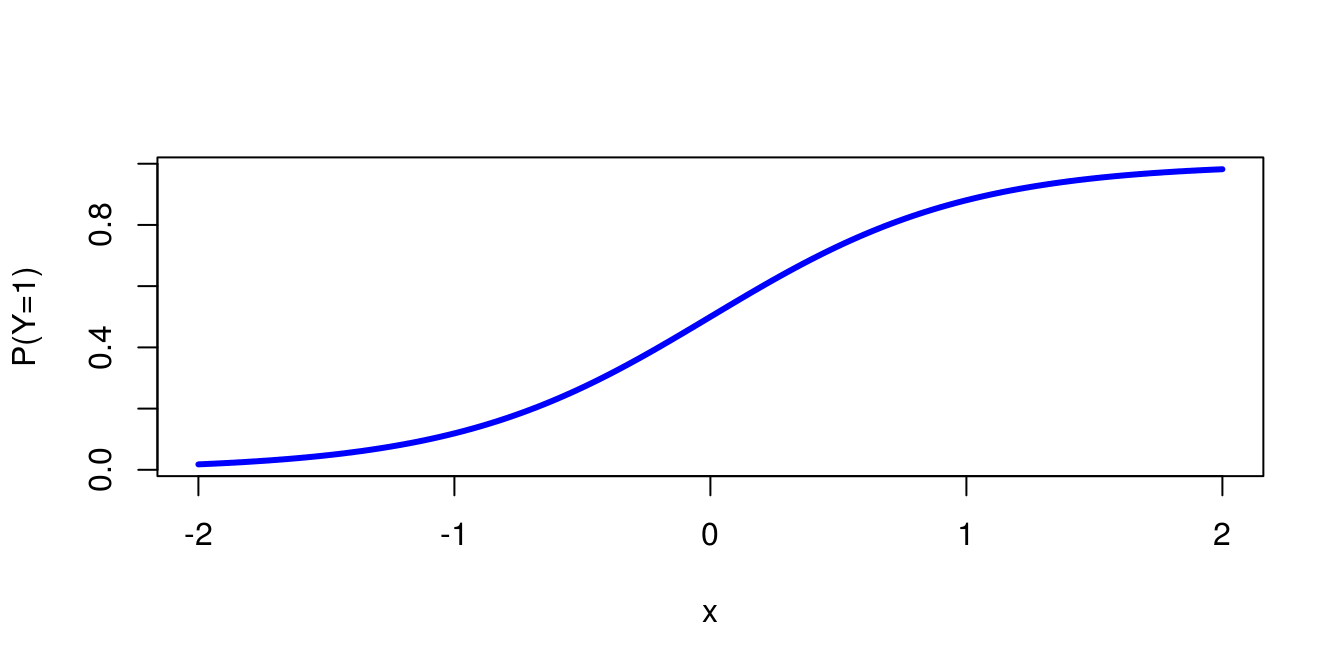
\includegraphics{_main_files/figure-latex/unnamed-chunk-5-1.pdf}

\subsubsection{Logit Model: Example 1}\label{logit-model-example-1}

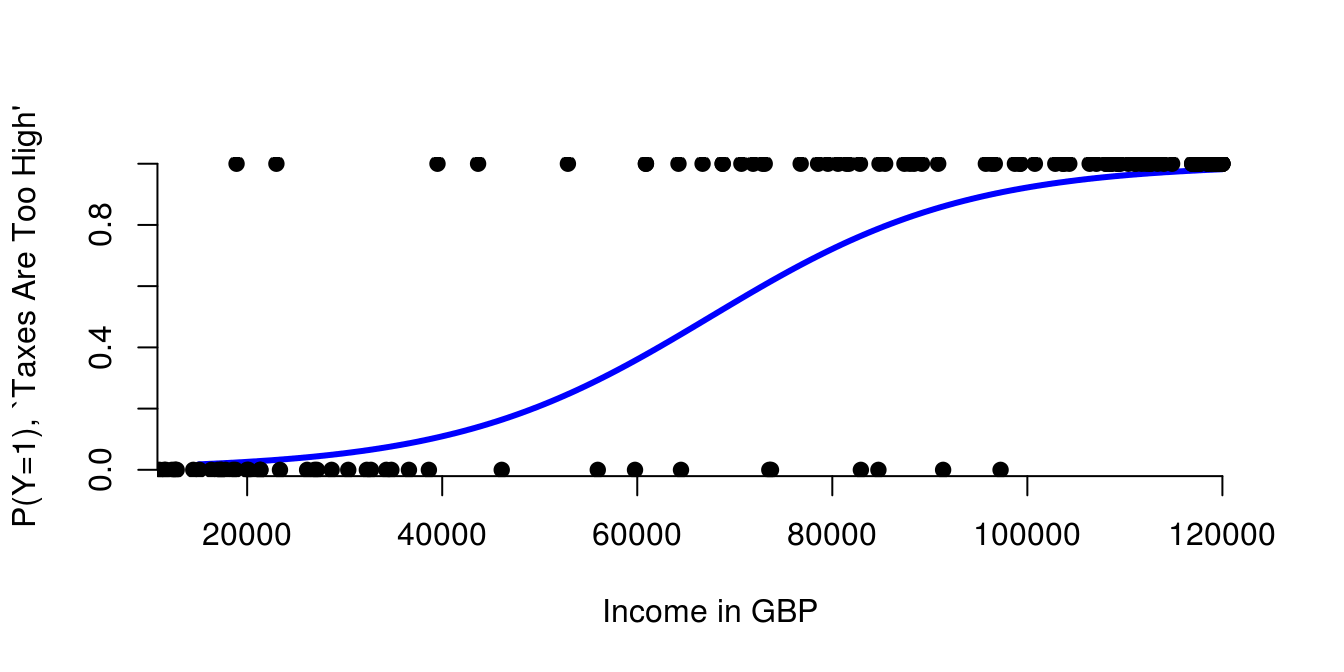
\includegraphics{_main_files/figure-latex/unnamed-chunk-6-1.pdf}

\begin{itemize}
\tightlist
\item
  We can make a prediction by calculating:
  \(P(y=1) = \frac{1}{1+\exp(-\beta_0 - \beta_1\cdot x)}\)
\end{itemize}

\subsubsection{Logit Model: Example 2}\label{logit-model-example-2}

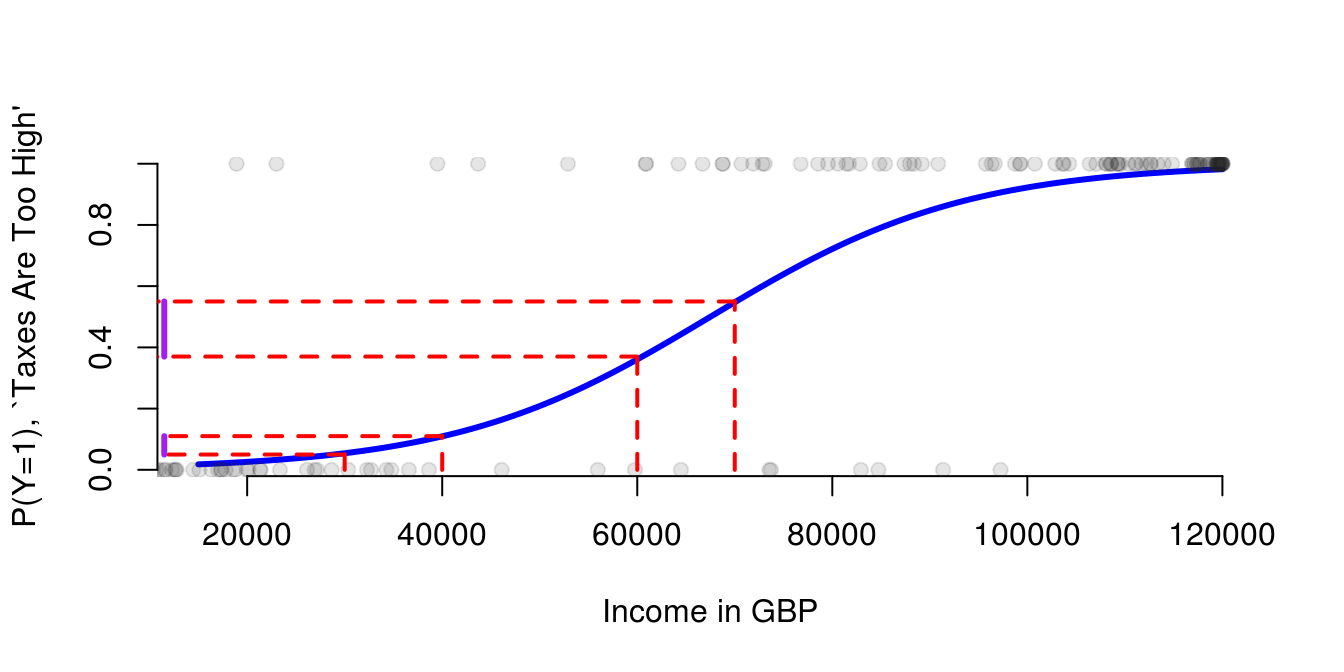
\includegraphics{_main_files/figure-latex/unnamed-chunk-7-1.pdf}

\begin{itemize}
\tightlist
\item
  Depending on where we add £1,000~we get a different marginal effect\\
  {[}\(\rightarrow\) because of our different functional form
  (s-shaped){]}\{\}
\end{itemize}

\subsubsection{Logit Model: Example 3}\label{logit-model-example-3}

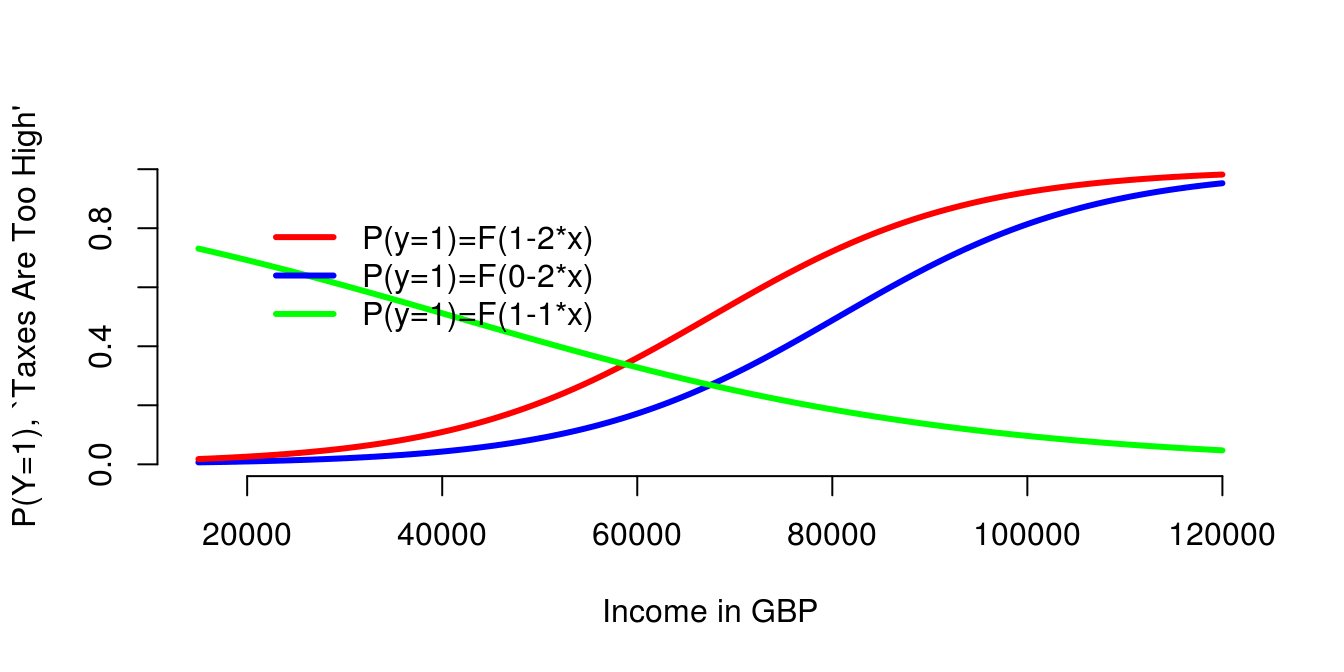
\includegraphics{_main_files/figure-latex/unnamed-chunk-8-1.pdf}

\begin{itemize}
\tightlist
\item
  A positive \(\beta_1\) makes the s-curve increase.
\item
  A smaller \(\beta_0\) shifts the s-curve to the right.
\item
  A negative \(\beta_1\) makes the s-curve decrease.
\end{itemize}

\section{Hands-on Tutorial}\label{hands-on-tutorial}

Let's start by loading the required packages:

\begin{Shaded}
\begin{Highlighting}[]
\KeywordTok{library}\NormalTok{(foreign) }
\KeywordTok{library}\NormalTok{(Zelig) }
\KeywordTok{library}\NormalTok{(texreg) }
\KeywordTok{library}\NormalTok{(lmtest)}
\KeywordTok{library}\NormalTok{(dplyr)}
\end{Highlighting}
\end{Shaded}

Clear the environment

\begin{Shaded}
\begin{Highlighting}[]
\KeywordTok{rm}\NormalTok{(}\DataTypeTok{list =} \KeywordTok{ls}\NormalTok{())}
\end{Highlighting}
\end{Shaded}

\subsection{Application to British Election Study
Dataset}\label{application-to-british-election-study-dataset}

We use a subset of the 2005 face-to-face British post election study to
explain turnout.

Disclaimer: We use a slightly modified version of the data set. For your
own research please visit the
\href{http://www.britishelectionstudy.com}{British Election Study
website} and download the original dataset.

You can download the dataset and codebook from the links below:

\begin{itemize}
\tightlist
\item
  \textbf{\href{http://uclspp.github.io/PUBLG100/data/bes.dta}{Dataset}}
\item
  \textbf{\href{http://uclspp.github.io/PUBLG100/data/bes_codebook.txt}{Codebook}}
\end{itemize}

Most of the variable names in the dataset are self explanatory, but ones
that need some clarification are listed below:

\begin{longtable}[c]{@{}lll@{}}
\toprule
\begin{minipage}[b]{0.19\columnwidth}\raggedright\strut
Variable
\strut\end{minipage} &
\begin{minipage}[b]{0.49\columnwidth}\raggedright\strut
Description
\strut\end{minipage} &
\begin{minipage}[b]{0.27\columnwidth}\raggedright\strut
Range
\strut\end{minipage}\tabularnewline
\midrule
\endhead
\begin{minipage}[t]{0.19\columnwidth}\raggedright\strut
Turnout
\strut\end{minipage} &
\begin{minipage}[t]{0.49\columnwidth}\raggedright\strut
Turnout at 2005 Brit election
\strut\end{minipage} &
\begin{minipage}[t]{0.27\columnwidth}\raggedright\strut
No (0); Yes (1)
\strut\end{minipage}\tabularnewline
\begin{minipage}[t]{0.19\columnwidth}\raggedright\strut
Gender
\strut\end{minipage} &
\begin{minipage}[t]{0.49\columnwidth}\raggedright\strut
R's gender
\strut\end{minipage} &
\begin{minipage}[t]{0.27\columnwidth}\raggedright\strut
1 (male); 0 (female)
\strut\end{minipage}\tabularnewline
\begin{minipage}[t]{0.19\columnwidth}\raggedright\strut
LeftRightSelf
\strut\end{minipage} &
\begin{minipage}[t]{0.49\columnwidth}\raggedright\strut
R's self placement on left-right
\strut\end{minipage} &
\begin{minipage}[t]{0.27\columnwidth}\raggedright\strut
1 (left) - 11 (right)
\strut\end{minipage}\tabularnewline
\begin{minipage}[t]{0.19\columnwidth}\raggedright\strut
CivicDutyIndex
\strut\end{minipage} &
\begin{minipage}[t]{0.49\columnwidth}\raggedright\strut
Sum of scores on CivicDuty1-7
\strut\end{minipage} &
\begin{minipage}[t]{0.27\columnwidth}\raggedright\strut
high values mean high civic duty
\strut\end{minipage}\tabularnewline
\begin{minipage}[t]{0.19\columnwidth}\raggedright\strut
polinfoindex
\strut\end{minipage} &
\begin{minipage}[t]{0.49\columnwidth}\raggedright\strut
Correctly answered knowledge questions
\strut\end{minipage} &
\begin{minipage}[t]{0.27\columnwidth}\raggedright\strut
0 (low) - 8 (high)
\strut\end{minipage}\tabularnewline
\begin{minipage}[t]{0.19\columnwidth}\raggedright\strut
edu*
\strut\end{minipage} &
\begin{minipage}[t]{0.49\columnwidth}\raggedright\strut
yrs of education
\strut\end{minipage} &
\begin{minipage}[t]{0.27\columnwidth}\raggedright\strut
binary
\strut\end{minipage}\tabularnewline
\begin{minipage}[t]{0.19\columnwidth}\raggedright\strut
in.school
\strut\end{minipage} &
\begin{minipage}[t]{0.49\columnwidth}\raggedright\strut
R still in school
\strut\end{minipage} &
\begin{minipage}[t]{0.27\columnwidth}\raggedright\strut
binary
\strut\end{minipage}\tabularnewline
\begin{minipage}[t]{0.19\columnwidth}\raggedright\strut
in.uni
\strut\end{minipage} &
\begin{minipage}[t]{0.49\columnwidth}\raggedright\strut
R attends university
\strut\end{minipage} &
\begin{minipage}[t]{0.27\columnwidth}\raggedright\strut
binary
\strut\end{minipage}\tabularnewline
\bottomrule
\end{longtable}

\subsection{Loading Data}\label{loading-data}

\begin{Shaded}
\begin{Highlighting}[]
\NormalTok{bes <-}\StringTok{ }\KeywordTok{read.dta}\NormalTok{(}\StringTok{"bes.dta"}\NormalTok{)}
\end{Highlighting}
\end{Shaded}

Let's convert the \texttt{Gender} variable to a factor to help us with
the interpretation of the results.

\begin{Shaded}
\begin{Highlighting}[]
\NormalTok{bes$Gender <-}\StringTok{ }\KeywordTok{factor}\NormalTok{(bes$Gender, }\DataTypeTok{levels =} \KeywordTok{c}\NormalTok{(}\DecValTok{0}\NormalTok{, }\DecValTok{1}\NormalTok{), }\DataTypeTok{labels =} \KeywordTok{c}\NormalTok{(}\StringTok{"Female"}\NormalTok{, }\StringTok{"Male"}\NormalTok{))}
\end{Highlighting}
\end{Shaded}

Now take a look at the first few observations to see what the dataset
looks like

\begin{Shaded}
\begin{Highlighting}[]
\KeywordTok{head}\NormalTok{(bes)}
\end{Highlighting}
\end{Shaded}

\begin{verbatim}
##   cs_id Turnout Vote2001 Income Age Gender PartyID Influence Attention
## 1     1       0        1      4  76 Female       1         1         8
## 2     2       1        1      5  32   Male       0         3         8
## 3     3       1       NA     NA  NA   <NA>      NA        NA        NA
## 4     4       0        1      1  35 Female       0         1         1
## 5     5       1        1      7  56   Male       0         1         9
## 6     6       1        1      4  76 Female       1         4         8
##   Telephone LeftrightSelf CivicDutyIndex polinfoindex edu15 edu16 edu17
## 1         1             7             20            7     1     0     0
## 2         1             6             15            5     0     1     0
## 3        NA            NA             NA           NA    NA    NA    NA
## 4         0             5             26            1     0     1     0
## 5         1             9             16            7     0     0     1
## 6         1             8             16            4     0     1     0
##   edu18 edu19plus in_school in_uni CivicDutyScores
## 1     0         0         0      0      -0.6331136
## 2     0         0         0      0       1.4794579
## 3    NA        NA        NA     NA              NA
## 4     0         0         0      0      -2.1466281
## 5     0         0         0      0       1.0324940
## 6     0         0         0      0       0.3658024
\end{verbatim}

We have a number of missing values. Let's remove them from the dataset
but we want to make sure we only remove observations when the variables
we are interested in are missing. We'll follow the same procedure we
used in week 5 for removing NA's.

While this method might seem tedious, it ensures that we're not dropping
observations unnecessarily.

\begin{Shaded}
\begin{Highlighting}[]
\NormalTok{bes <-}\StringTok{ }\KeywordTok{filter}\NormalTok{(bes, }
              \NormalTok{!}\KeywordTok{is.na}\NormalTok{(Turnout), }
              \NormalTok{!}\KeywordTok{is.na}\NormalTok{(Income), }
              \NormalTok{!}\KeywordTok{is.na}\NormalTok{(polinfoindex), }
              \NormalTok{!}\KeywordTok{is.na}\NormalTok{(Gender), }
              \NormalTok{!}\KeywordTok{is.na}\NormalTok{(edu15), }
              \NormalTok{!}\KeywordTok{is.na}\NormalTok{(edu17), }
              \NormalTok{!}\KeywordTok{is.na}\NormalTok{(edu18), }
              \NormalTok{!}\KeywordTok{is.na}\NormalTok{(edu19plus), }
              \NormalTok{!}\KeywordTok{is.na}\NormalTok{(in_school), }
              \NormalTok{!}\KeywordTok{is.na}\NormalTok{(in_uni))}
\end{Highlighting}
\end{Shaded}

\subsection{Regression with a Binary Dependent
Variable}\label{regression-with-a-binary-dependent-variable}

We use the generalized linear model function \texttt{glm()} to estimate
a logistic regression. The syntax is very similar to other regression
functions we're already familiar with, for example \texttt{lm()} and
\texttt{plm()}. The \texttt{glm()} function can be used to estimate many
different models. We tell \texttt{glm()} that we've binary dependent
variable and we want to use the cumulative logistic link function using
the \texttt{family\ =\ binomial(link\ =\ "logit")} argument:

\begin{Shaded}
\begin{Highlighting}[]
\NormalTok{model1 <-}\StringTok{ }\KeywordTok{glm}\NormalTok{(Turnout ~}\StringTok{ }\NormalTok{Income +}\StringTok{ }\NormalTok{polinfoindex +}\StringTok{ }\NormalTok{Gender +}\StringTok{ }
\StringTok{                }\NormalTok{edu15 +}\StringTok{ }\NormalTok{edu17 +}\StringTok{ }\NormalTok{edu18 +}\StringTok{ }\NormalTok{edu19plus +}\StringTok{ }\NormalTok{in_school +}\StringTok{ }\NormalTok{in_uni, }
              \DataTypeTok{family =} \KeywordTok{binomial}\NormalTok{(}\DataTypeTok{link =} \StringTok{"logit"}\NormalTok{),}
              \DataTypeTok{data =} \NormalTok{bes)}

\KeywordTok{screenreg}\NormalTok{(model1)}
\end{Highlighting}
\end{Shaded}

\begin{verbatim}
## 
## ============================
##                 Model 1     
## ----------------------------
## (Intercept)        -1.14 ***
##                    (0.15)   
## Income              0.03    
##                    (0.02)   
## polinfoindex        0.38 ***
##                    (0.02)   
## GenderMale         -0.35 ***
##                    (0.08)   
## edu15               0.38 ***
##                    (0.10)   
## edu17               0.46 ** 
##                    (0.15)   
## edu18               0.11    
##                    (0.14)   
## edu19plus           0.24 *  
##                    (0.12)   
## in_school           0.15    
##                    (0.39)   
## in_uni             -0.72 ** 
##                    (0.25)   
## ----------------------------
## AIC              4401.20    
## BIC              4464.53    
## Log Likelihood  -2190.60    
## Deviance         4381.20    
## Num. obs.        4161       
## ============================
## *** p < 0.001, ** p < 0.01, * p < 0.05
\end{verbatim}

\subsection{Model Quality}\label{model-quality}

To assess the predictive accuracy of our model we will check the
percentage of cases that it correctly predicts. Let's look the turnout
data first. According to the codebook, \texttt{0} means the person did
not vote, and \texttt{1} means they voted.

\begin{Shaded}
\begin{Highlighting}[]
\KeywordTok{table}\NormalTok{(bes$Turnout) }
\end{Highlighting}
\end{Shaded}

\begin{verbatim}
## 
##    0    1 
## 1079 3082
\end{verbatim}

If we look at the mean of Turnout we will see that is \texttt{0.74}.
That means \texttt{74.07\%} of the respondents said that they turned out
to vote. If you predict for every respondent that they voted, you will
be right for \texttt{74.07\%} of the people. That is the naive guess and
the benchmark for our model. If we predict more than \texttt{74.07\%} of
cases correctly our model adds value.

Below we will estimate predicted probabilities for each observation.
That is, the probability our model assigns that a respondent will turn
out to vote for every person in our data. To do so we use the
\texttt{predict()} function with the following the usage syntax:

\begin{verbatim}
predict(model, type = "response")
\end{verbatim}

Type \texttt{help(predict.glm)} for information on all arguments.

\begin{Shaded}
\begin{Highlighting}[]
\NormalTok{predicted_probs <-}\StringTok{ }\KeywordTok{predict}\NormalTok{(model1, }\DataTypeTok{type =} \StringTok{"response"}\NormalTok{)}
\end{Highlighting}
\end{Shaded}

Now that we have assigned probabilities to people turning out to vote,
we have to translate those into outcomes. Turnout is binary. A
straightforward way would be to say: we predict that all people with a
predicted probability above \texttt{50\%} vote and all with predicted
probabilities below or equal to \texttt{50\%} abstain.

Using the \texttt{50\%} threshold, we create a new variable
\texttt{expected\_values} that is \texttt{1} if our predicted
probability is larger than \texttt{0.5} and \texttt{0} otherwise.

\begin{Shaded}
\begin{Highlighting}[]
\NormalTok{expected <-}\StringTok{ }\KeywordTok{as.numeric}\NormalTok{(predicted_probs >}\StringTok{ }\FloatTok{0.5}\NormalTok{)}
\end{Highlighting}
\end{Shaded}

NOTE: The condition \texttt{predicted\_probs\ \textgreater{}\ 0.5} gives
us \texttt{FASLE/TRUE}, but since our dataset uses \texttt{0/1} for the
\texttt{Turnout} variable, we convert it to a numeric value using
\texttt{as.numeric()} function.

All we have to do now is to compare our expected values of turnout
against the actually observed values of turnout. We want our predictions
to coincide with the actually observed outcomes. But we need to be aware
of two types of errors we can make:

\begin{longtable}[c]{@{}ll@{}}
\toprule
\begin{minipage}[t]{0.50\columnwidth}\raggedright\strut
- A type I error is a false positive. It is like crying wolf when there
is nothing there (we mistakenly reject a true null hypothesis). - A type
II error is a false negative. It is like not noticing the wolf and
finding all your sheep dead the next morning (we fail to reject a false
null hypothesis).
\strut\end{minipage} &
\begin{minipage}[t]{0.43\columnwidth}\raggedright\strut
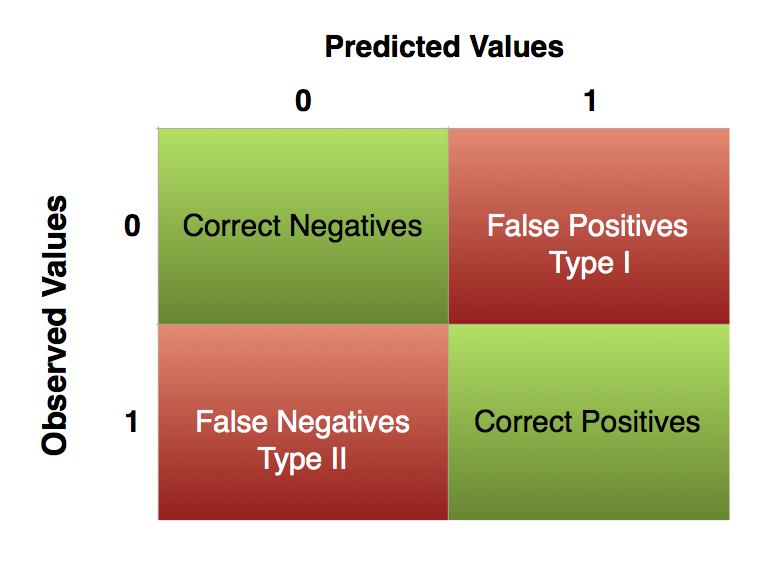
\includegraphics{./img/confusion_matrix.png}
\strut\end{minipage}\tabularnewline
\bottomrule
\end{longtable}

The threshold that we set is directly related to the proportion of type
I to type II errors. Increasing the threshold will reduce the number of
false positives but increase the number of false negatives and vice
versa. The default choice is a threshold of \texttt{0.5}. However, you
may imagine situations where one type of error is more costly than the
other. For example, given the cost of civil wars, a model predicting
civil war may focus on reducing false negatives at the cost of a larger
fraction of false positives.

We proceed by producing a table of predictions against actual outcomes.
With that we will calculate the percentage of correctly predicted cases
and compare that to the naive guess. We have the actually observed cases
in our dependent variable (\texttt{Turnout}). The table is just a
frequency table. The percentage of correctly predicted cases is simply
the sum of correctly predicted cases over the number of cases.

\begin{Shaded}
\begin{Highlighting}[]
\NormalTok{observed <-}\StringTok{ }\NormalTok{bes$Turnout}

\NormalTok{outcome <-}\StringTok{ }\KeywordTok{table}\NormalTok{(observed,expected)}
\NormalTok{outcome}
\end{Highlighting}
\end{Shaded}

\begin{verbatim}
##         expected
## observed    0    1
##        0  160  919
##        1  108 2974
\end{verbatim}

Now let's find out how many we correctly predicted and how many we got
wrong. You can manually add the numbers if you want, but it's simple
enough to take the values out of the 2x2 table:

\begin{itemize}
\tightlist
\item
  Correct negatives are in row \texttt{1}, column \texttt{1}
\item
  Correct positives are in row \texttt{2}, column \texttt{2}
\item
  All others are incorrect
\end{itemize}

\begin{Shaded}
\begin{Highlighting}[]
\NormalTok{(outcome[}\DecValTok{1}\NormalTok{,}\DecValTok{1}\NormalTok{] +}\StringTok{ }\NormalTok{outcome[}\DecValTok{2}\NormalTok{,}\DecValTok{2}\NormalTok{]) /}\StringTok{ }\KeywordTok{sum}\NormalTok{(outcome)}
\end{Highlighting}
\end{Shaded}

\begin{verbatim}
## [1] 0.7531843
\end{verbatim}

Now let's remember what the actual turnout was:

\begin{Shaded}
\begin{Highlighting}[]
\KeywordTok{table}\NormalTok{(bes$Turnout)}
\end{Highlighting}
\end{Shaded}

\begin{verbatim}
## 
##    0    1 
## 1079 3082
\end{verbatim}

In order to calculate the naive guess, we simply divide the mode by the
total number of observations

\begin{Shaded}
\begin{Highlighting}[]
\DecValTok{3082} \NormalTok{/}\StringTok{ }\NormalTok{(}\DecValTok{1079} \NormalTok{+}\StringTok{ }\DecValTok{3082}\NormalTok{)}
\end{Highlighting}
\end{Shaded}

\begin{verbatim}
## [1] 0.7406873
\end{verbatim}

You can see that our model outperforms the naive guess slightly. The
more lopsided the distribution of your binary dependent variable, the
harder it is to build a successful model.

\subsubsection{Joint hypothesis testing}\label{joint-hypothesis-testing}

We will add two more explanatory variables to our model:
\texttt{Influence} and \texttt{Age}. \texttt{Influence} corresponds to a
theory we want to test while \texttt{Age} is a socio-economic control
variable.

We want to test two theories: the rational voter model and the resource
theory.

\begin{itemize}
\item
  Influence operationalises a part of the rational voter theory. In that
  theory citizens are more likely to turnout the more they belive that
  their vote matters. The variable \texttt{Influence} measures the
  subjective feeling of being able to influence politics.
\item
  The variables \texttt{Income} and \texttt{polinfoindex} correspond to
  a second theory which states that people who have more cognitive and
  material resources are more likely to participate in politics.
\end{itemize}

Depending on whether the coefficients corresponding to the respective
theories are significant or not, we can say something about whether
these theories help to explain turnout.

The remaining variables for gender, education and the added variable
\texttt{Age} are socio-economic controls. We added age because previous
research has shown that political participation changes with the life
cycle.

\begin{Shaded}
\begin{Highlighting}[]
\NormalTok{model2 <-}\StringTok{ }\KeywordTok{glm}\NormalTok{(Turnout ~}\StringTok{ }\NormalTok{Income +}\StringTok{ }\NormalTok{polinfoindex +}\StringTok{ }\NormalTok{Influence +}\StringTok{ }\NormalTok{Gender +}\StringTok{ }\NormalTok{Age +}\StringTok{ }
\StringTok{                }\NormalTok{edu15 +}\StringTok{ }\NormalTok{edu17 +}\StringTok{ }\NormalTok{edu18 +}\StringTok{ }\NormalTok{edu19plus +}\StringTok{ }\NormalTok{in_school +}\StringTok{ }\NormalTok{in_uni, }
              \DataTypeTok{family =} \KeywordTok{binomial}\NormalTok{(}\DataTypeTok{link =} \StringTok{"logit"}\NormalTok{), }\DataTypeTok{data =} \NormalTok{bes)}

\KeywordTok{screenreg}\NormalTok{(}\KeywordTok{list}\NormalTok{(model1, model2))}
\end{Highlighting}
\end{Shaded}

\begin{verbatim}
## 
## ==========================================
##                 Model 1       Model 2     
## ------------------------------------------
## (Intercept)        -1.14 ***     -3.90 ***
##                    (0.15)        (0.22)   
## Income              0.03          0.15 ***
##                    (0.02)        (0.02)   
## polinfoindex        0.38 ***      0.25 ***
##                    (0.02)        (0.02)   
## GenderMale         -0.35 ***     -0.36 ***
##                    (0.08)        (0.08)   
## edu15               0.38 ***     -0.34 ** 
##                    (0.10)        (0.11)   
## edu17               0.46 **       0.36 *  
##                    (0.15)        (0.16)   
## edu18               0.11          0.14    
##                    (0.14)        (0.15)   
## edu19plus           0.24 *        0.01    
##                    (0.12)        (0.13)   
## in_school           0.15          1.13 ** 
##                    (0.39)        (0.40)   
## in_uni             -0.72 **      -0.05    
##                    (0.25)        (0.27)   
## Influence                         0.21 ***
##                                  (0.02)   
## Age                               0.05 ***
##                                  (0.00)   
## ------------------------------------------
## AIC              4401.20       4003.90    
## BIC              4464.53       4079.90    
## Log Likelihood  -2190.60      -1989.95    
## Deviance         4381.20       3979.90    
## Num. obs.        4161          4161       
## ==========================================
## *** p < 0.001, ** p < 0.01, * p < 0.05
\end{verbatim}

The variables corresponding to the resource theory are \texttt{Income}
and \texttt{polinfoindex}. In our model 2 (the one we interpret), both
more income and more interest in politics are related to a higher
probability to turn out to vote. That is in line with the theory.
Interestingly, income was previously insignificant in model 1. It is
quite likely that model 1 suffered from omitted variable bias.

As the rational voter model predicts, a higher subjective probability to
cast a decisive vote, which we crudly proxy by the feeling to be able to
influence politics, does correspond to a higher probability to vote as
indicated by the positive significant effect of our \texttt{Influence}
variable.

We will test if model 2 does better at predicting turnout than model 1.
We use the likelihood ratio test. This is warranted because we added two
variables and corresponds to the F-test in the OLS models estimated
before. You can see values for the logged likelihood in the regression
table. You cannot in general say whether a value for the likelihood is
small or large but you can use it to compare models that are based on
the same sample. A larger log-likelihood is better. Looking at the
regression table we see that the log-likelihood is larger in model 2
than in model 1.

We use the \texttt{lrtest()} function from the \texttt{lmtest} package
to test whether that difference is statistically significant. The syntax
is the following:

\begin{Shaded}
\begin{Highlighting}[]
\KeywordTok{lrtest}\NormalTok{(model1, model2)}
\end{Highlighting}
\end{Shaded}

\begin{verbatim}
## Likelihood ratio test
## 
## Model 1: Turnout ~ Income + polinfoindex + Gender + edu15 + edu17 + edu18 + 
##     edu19plus + in_school + in_uni
## Model 2: Turnout ~ Income + polinfoindex + Influence + Gender + Age + 
##     edu15 + edu17 + edu18 + edu19plus + in_school + in_uni
##   #Df  LogLik Df Chisq Pr(>Chisq)    
## 1  10 -2190.6                        
## 2  12 -1990.0  2 401.3  < 2.2e-16 ***
## ---
## Signif. codes:  0 '***' 0.001 '**' 0.01 '*' 0.05 '.' 0.1 ' ' 1
\end{verbatim}

The p-value in the likelihood ratio test is smaller than \texttt{0.05}.
Therefore, the difference between the two log-likelihoods is
statistically significant which means that model 2 is better at
explaining turnout.

Now let's see if AIC and BIC agree.

\begin{Shaded}
\begin{Highlighting}[]
\KeywordTok{AIC}\NormalTok{(model1, model2)}
\end{Highlighting}
\end{Shaded}

\begin{verbatim}
##        df      AIC
## model1 10 4401.200
## model2 12 4003.901
\end{verbatim}

\begin{Shaded}
\begin{Highlighting}[]
\KeywordTok{BIC}\NormalTok{(model1, model2) }
\end{Highlighting}
\end{Shaded}

\begin{verbatim}
##        df      BIC
## model1 10 4464.535
## model2 12 4079.903
\end{verbatim}

According to both AIC and BIC, model 2 has a better fit.

\section{Exercises}\label{exercises}

\begin{itemize}
\tightlist
\item
  \textbf{\href{http://uclspp.github.io/PUBLG100/data/mroz.dta}{Dataset}}
\item
  \textbf{\href{http://uclspp.github.io/PUBLG100/data/mroz.txt}{Codebook}}
\end{itemize}

\begin{enumerate}
\def\labelenumi{\arabic{enumi}.}
\item
  Select at least 4 predictors (including \texttt{age} but excluding
  \texttt{exper}) to explain women in the labor force and provide
  theoretical justification for your selection.
\item
  Estimate a model using the predictors you selected, present your
  findings and provide an assessment of the model quality.
\item
  Does the addition of \texttt{exper} to your model improve its
  predictive performance?
\item
  Based on your model, what's the probability of a 40 year old woman
  with 12 years of experience to be in the labor force? Make sure to
  include a confidence interval for your prediction.
\item
  Compare the effects of experience in the labor market on the outcome
  variable under two hypothetical scenarios:

  \begin{itemize}
  \tightlist
  \item
    A woman with age in the 25th percentile
  \item
    A woman with age in the 75th percentile
  \end{itemize}
\item
  Provide a visualization to illustrate your findings.
\end{enumerate}

Reference: Mroz, T.A. (1987): ``The Sensitiviy of an Empirical Model of
Married Women's Hours of Work to Economic and Statistical Assumptions'',
Econometrica, 55, 765-799.

\end{document}
